\documentclass[a4paper,10pt,captions=tableheading,DIV=14]{scrartcl}
\pdfoutput=1
\bibliographystyle{utphys27mod}

% ----------------------------------------------------------- Packages
\usepackage{amsmath,amssymb,url,cite,slashed,cancel,booktabs,hyperref,graphicx,xspace,subcaption}
\usepackage[capitalize]{cleveref}
%%%UNUSED%%% \usepackage{feynmp,enumerate,multirow,wrapfig}
\renewcommand\citepunct{,\penalty1000\hskip.13emplus.1emminus.1em\relax} % no line-break in \cite
\renewcommand\thefootnote{*\arabic{footnote}}
\numberwithin{equation}{section}
% COMMENTS
\newcommand{\comment}[1]{{\textbf{\small \color{red} [#1]}}}
\newcommand{\cmark}{\ding{51}} % check mark
\newcommand{\xmark}{\ding{55}} % X mark

% MATH NOTATION
\newcommand\w[1]{_{\mathrm{#1}}}
\newcommand\vc[1]{{\boldsymbol{#1}}}
\newcommand\dd{\mathop{}\!\mathrm{d}}
\newcommand\DD{\mathop{}\!\mathrm{D}}
\newcommand\ee{\mathop{}\!\mathrm{e}}
\newcommand\abs[1]{\lvert#1\rvert}
\newcommand\norm[1]{\lVert#1\rVert}
\newcommand\Abs[1]{\left\lvert#1\right\rvert}
\newcommand\Norm[1]{\left\lVert#1\right\rVert}
\newcommand\ii{\mathrm{i}}
\newcommand\co[1]{\mathrm{c}_{#1}}
\newcommand\si[1]{\mathrm{s}_{#1}}
\newcommand\coco[1]{\mathrm{c}^2_{#1}}
\newcommand\sisi[1]{\mathrm{s}^2_{#1}}
\newcommand\pmat[1]{\begin{pmatrix}#1\end{pmatrix}}
\DeclareMathOperator{\Order}{\mathcal{O}}
\DeclareMathOperator{\sign}{\mathrm{sign}}
\DeclareMathOperator{\ddelta}{\delta}
\DeclareMathOperator{\Tr}{\mathrm{Tr}}
\DeclareMathOperator{\diag}{\mathrm{diag}}
\renewcommand{\Re}{\mathop{\mathrm{Re}}}
\renewcommand{\Im}{\mathop{\mathrm{Im}}}

\newcommand\oneone{1}
\newcommand{\dn}[3]{\frac{\dd^#1 #2}{\dd #3^#1}}    % derivatives
\newcommand{\pdn}[3]{\frac{\partial^#1 #2}{\partial #3^#1}}
\newcommand{\pd}[2]{\frac{\partial #1}{\partial #2}}
\newcommand\parenfrac[3]{\def\temp{#3}\Bigl(\frac{#1}{#2}\Bigr)\ifx\oneone\temp\relax\relax\else^{#3}\fi}
\newcommand\vev[1]{\langle#1\rangle}
\newcommand{\mean}[1]{\left\langle #1 \right\rangle}

\newcommand\hc{\text{h.c.}}

% units
\newcommand\unit[1]{\,\mathrm{#1}\xspace}
\newcommand\eV{\unit{eV}}
\newcommand\keV{\unit{keV}}
\newcommand\MeV{\unit{MeV}}
\newcommand\GeV{\unit{GeV}}
\newcommand\TeV{\unit{TeV}}
\newcommand\PeV{\unit{PeV}}
\newcommand\fb{\unit{fb}}
\newcommand\pb{\unit{pb}}
\newcommand\iab{\unit{ab^{-1}}}
\newcommand\ifb{\unit{fb^{-1}}}
\newcommand\ipb{\unit{pb^{-1}}}
\newcommand\fm{\unit{fm}}


% scientific form of numbers
\makeatletter
\def\EE{\@ifnextchar-{\@@EE}{\@EE}}
\def\@EE#1{\ifnum#1=1 \times\!10 \else \times\!10^{#1}\fi}
\def\@@EE#1#2{\times\!10^{-#2}}
\makeatother

% ---------------------------------------------------- For Sho's Notes
\usepackage{scrlayer-scrpage,color,soul}
\usepackage[hhmmss]{datetime}
\newdateformat{mydate}{\THEDAY\;\shortmonthname.\;\THEYEAR}
\addtokomafont{pagehead}{\small\normalfont}
\ohead{\texttt{[\jobname~@~\mydate\today~\currenttime]}}
\bibliographystyle{utphys27mod}

% --- minted experimental
\usepackage{ifplatform,listings}
\lstset{columns=[l]fullflexible,basicstyle=\small\ttfamily,xleftmargin=2em,frame=L,keepspaces=true}
\ifshellescape
\usepackage{minted}
\setminted{linenos,xleftmargin=7\fboxsep,breaklines,fontsize=\small,frame=leftline,stepnumber=5,framesep=2\fboxsep,escapeinside=||,mathescape=true}
\setminted[console]{xleftmargin=6\fboxsep,frame=none}
\else
\makeatletter
\lstnewenvironment{minted}[1]
  {\csname\@lst @SetFirstNumber\endcsname}
  {\csname\@lst @SaveFirstNumber\endcsname}
\makeatother
\fi
% ---

\newcommand{\mathfunc}[2]{\mathcmd{#1}\texttt{[}\matharg{#2}\texttt{]}}
\newcommand{\mathcmd}[1]{\textup{\texttt{#1}}}
\newcommand{\mathtext}[1]{\textup{\texttt{"#1"}}}
\newcommand{\matharg}[1]{\textsl{#1}}

\newcommand{\TODO}[1]{{\textbf{\lstset{}\color{red}$\clubsuit$#1}}}

% commands for this document
\definecolor{navy}{rgb}{0,0,0.5}
\newcommand\Damu{\Delta a_\mu}
\newcommand\amu[1][\relax]{\ifx#1\relax{a_\mu}\else{a_\mu^{\mathrm{#1}}}\fi}
\newcommand\smu{\tilde\mu}
\newcommand\smuL{\tilde\mu\w L}
\newcommand\smuR{\tilde\mu\w R}
\newcommand\neut  [1][\relax]{{\tilde\chi^0_{#1}}}
\newcommand\charP [1][\relax]{{\tilde\chi^+_{#1}}}
\newcommand\charM [1][\relax]{{\tilde\chi^-_{#1}}}
\newcommand\charPM[1][\relax]{{\tilde\chi^\pm_{#1}}}
\newcommand\file[1]{\lstinline[basicstyle=\ttfamily\color{navy}]{#1}}
\newcommand\package[2][\relax]{\texttt{#2}\ifx#1\relax\relax\else~\texttt{#1}\fi}


\author{Sho Iwamoto}
\title{Analysis description}
\begin{document}
%\maketitle
\begin{center}{\makeatletter
{\huge\usekomafont{title}\@title}\par\vspace{2em}
{\Large \@author}\par\vspace{2em}
}
\begin{abstract}\noindent
This document serves for the description of my analysis codes as well as reference base through the bibliography file.
\end{abstract}
\end{center}

%---------------------------------------------------------------------
\section{Code base}
This repository is managed as a git repository.
A special directory \file{/vendor} is prepared to handle external packages, which are prepared as git-submodules or python packages.
Packages provided as git-submodules are installed by
\begin{minted}{console}
$ git submodule init
$ git submodule update
$ git submodule status   # to list the submodules
\end{minted}
The packages are installed under \file{/vendor} and some of them needs \texttt{make} etc.

These installation steps are compiled in \file{/vendor/makefile}.

External python packages are installed by
\begin{minted}{console}
$ pip install -r vendor/requirements.txt
\end{minted}
but some of them are only for Python~3, while MadGraph~5 is only for Python~2.
To solve this issue, users may have to use some technology such as \texttt{pyenv}.
In addition, they may want to use \texttt{pyenv-virtualenv} to isolate the python packages used for this project (i.e., installed by the above command).
Unfortunately this document does not cover the usage of \texttt{pyenv}, as it depends on users' environment (and also because there are many other literature).


These installation steps are compiled in \file{/vendor/makefile}.


\section{Spectrum}

We assume that the colored superparticles and extra Higgs bosons are decoupled, and that the slepton flavor is conserved.
The superparticles available at the LHC is thus neutralinos, charginos, and sleptons, whose mass spectrum is given by $(M_1, M_2, \mu, \tan\beta)$, slepton soft masses $(m\w L)_{i}$ and $(m\w R)_{i}$, and slepton trilinear terms $(A_e)_{i}$.

We consider the MSSM scenarios with the WHL contribution to $\amu$ dominating over the other SUSY contributions, which is realized if $(m\w L)_2\ll (m\w R)_2$, i.e., $\smuR$ is much heavier than $\smuL$.
We thus fix our parameters as, also for the sake of simplicity,
\begin{align}
 M_1 & =\frac12 M_2, &
 \tan\beta &= 40, &
 A_e & = 0, &
 m\w L & \text{ is flavor independent}, &
 m\w R & = 3\TeV,
\end{align}
and take $(M_2, m\w L, \mu)$ as the three parameters.

The MSSM parameters (mass spectrum and mixing matrices) are calculated at the tree-level.
Decay rates of SUSY particles are calculated by \package[1.5a]{SUSY-HIT} (namely \package[1.5a]{SDECAY}).
The Higgs boson mass is fixed to $125.0\GeV$ and the decay rates are taken from the CERN yellow report.
The other Standard Model parameters are taken from PDG2019.

The value of $\amu[MSSM]$ is calculated by \package[1.5]{GM2Calc} with $\tan\beta$ resummation but at the one-loop level so that the value is free from the mass of the decoupled particles, while it is dependent on $m\w R$.
Considering that $\amu[MSSM]$ is approximated by the mass insertion technique as
\begin{equation}
 \amu[MSSM]\simeq \amu[WHL1]+\amu[WHL2]+\amu[BHL]+\amu[BHR]+\amu[BLR],
\end{equation}
we also define an approximated value of $\amu[MSSM]$ as
\begin{equation}
 \amu[MI]:=\amu[WHL1] + \amu[WHL2] + \amu[BHL],
\end{equation}
which is independent of $m\w R$.

Accordingly, our estimation of $\amu[MSSM]$ is subject to uncertainty coming from (a) loop-level corrections to the mass and mixings, (b) two-loop level calculation of $\amu[MSSM]$, and (c) from the unknown $m_{\smuR}$.
(a) and (b) is related to the unknown masses of colored SUSY particles and heavy Higgs bosons.
We may estimate the magnitude of (c) as the difference between $\amu[MSSM]$ and $\amu[MI]$.


The directory \file{/spectrum} contains the scripts for spectrum generation and the generated spectrum files.
Mathematica package \file{gm2grid.wl} defines our low-energy input and calculate $\amu[MI]$ and $\amu[MSSM]$, internally calling \package{GM2Calc}.
\file{gen\_grid.wls} is the script to generate our grid tables \file{*.in}, in which we have three ``table'' definitions:
\begin{align}
 \text{\texttt{tab1}}&: \mu/M_2 = 1&
 \text{\texttt{tab2}}&: \mu/M_2 = 2&
 \text{\texttt{tab3}}&: \mu/M_2 = 3/4
\end{align}
The respective grid (as well as the model points with desired $x$) are generated by
\begin{minted}{console}
$ ./gen_grid.wls grid tab1
$ ./gen_grid.wls grid tab2
$ ./gen_grid.wls grid tab3
$ ./gen_grid.wls x005 tab1 0.05
$ ./gen_grid.wls x005 tab2 0.05
$ ./gen_grid.wls x005 tab3 0.05
$ ./gen_grid.wls x050 tab1 0.5
$ ./gen_grid.wls x050 tab2 0.5
$ ./gen_grid.wls x050 tab3 0.5
$ ./gen_grid.wls x095 tab1 0.95
$ ./gen_grid.wls x095 tab2 0.95
$ ./gen_grid.wls x095 tab3 0.95
\end{minted}
where
\begin{equation}
 x=\frac{m_{\smuL} - m_{\neut[1]}}{m_{\charPM[1]} - m_{\neut[1]}}.
\end{equation}

Then my inter-project package \href{https://github.com/misho104/SimSUSY/tree/master/simsusy}{\texttt{GitHub:misho104/simsusy}} calculate the masses and mixings at the tree-level to output \file{*.spec}.
The \file{.spec} files are passed to \package{SUSY-HIT} to generate \file{*.sdecay} files.
We then patch these files to give correct Higgs mass etc.\ and the final \file{*.slha} files are obtained.

The \file{*.slha} files have two special blocks:
\begin{minted}{text}
BLOCK SPHENOLOWENERGY
    21     1.39494693E-08   # |$\amu[MSSM]$ by GM2Calc|
BLOCK GM2MASSINSERTION
     1     1.31429479E-08   # WHL contribution |$\amu[WHL1]+\amu[WHL2]$|
     2     1.11890140E-11   # BLR contribution |$\amu[BLR]$|
     3    -5.15866472E-13   # BHR contribution |$\amu[BHR]$|
     4     7.04543437E-10   # BHL contribution |$\amu[BHL]$|
\end{minted}

\Cref{fig:spectra} shows the important properties of the spectra generated by \file{plots/plot_spectrum.wls}.



\begin{figure}[p]
\begin{subfigure}[b]{\textwidth}
 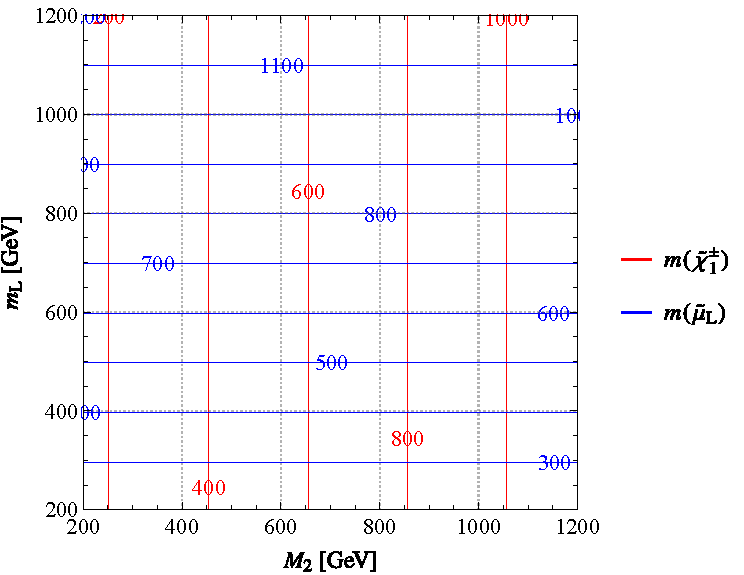
\includegraphics[scale=0.6]{../plots/plot_spectrum_tab1_massplot.pdf}
\hfill
 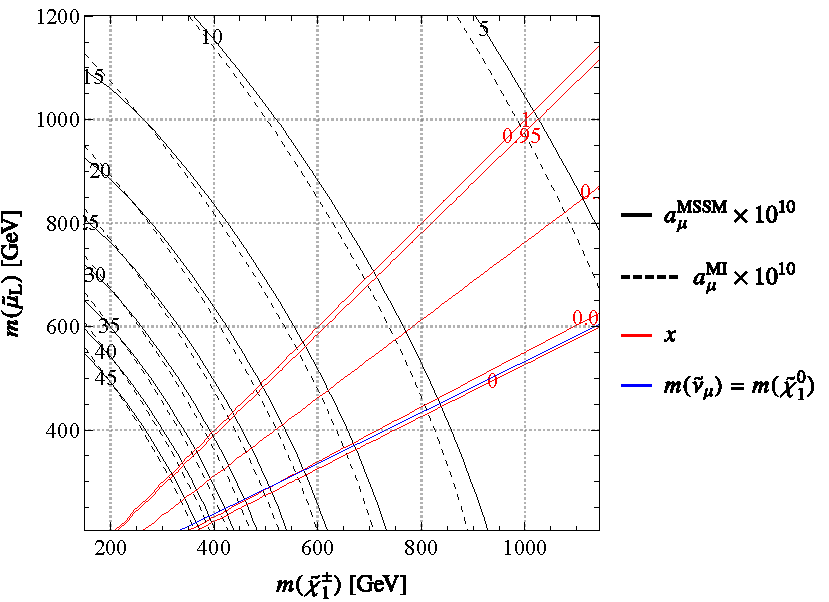
\includegraphics[scale=0.6]{../plots/plot_spectrum_tab1_physplot.pdf}
\caption{\label{fig:spectra-tab1} For $\mu=M_2$.}
\end{subfigure}

\vspace{1em}

\begin{subfigure}[b]{\textwidth}
 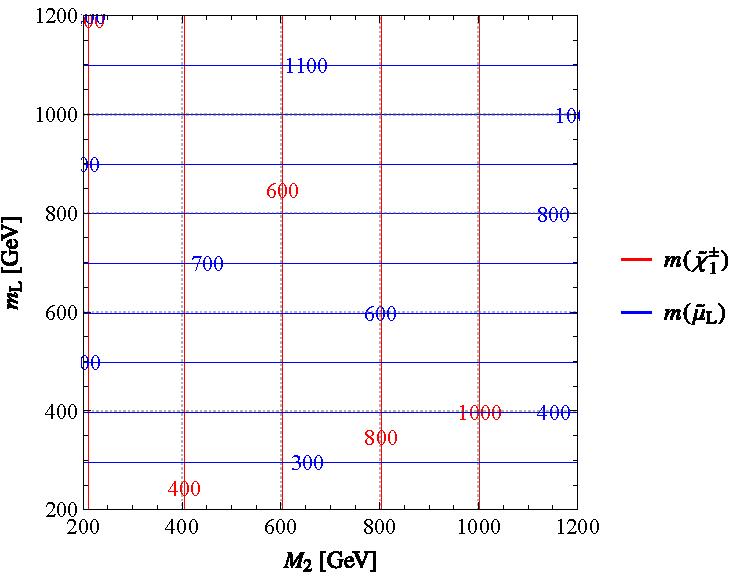
\includegraphics[scale=0.6]{../plots/plot_spectrum_tab2_massplot.pdf}
\hfill
 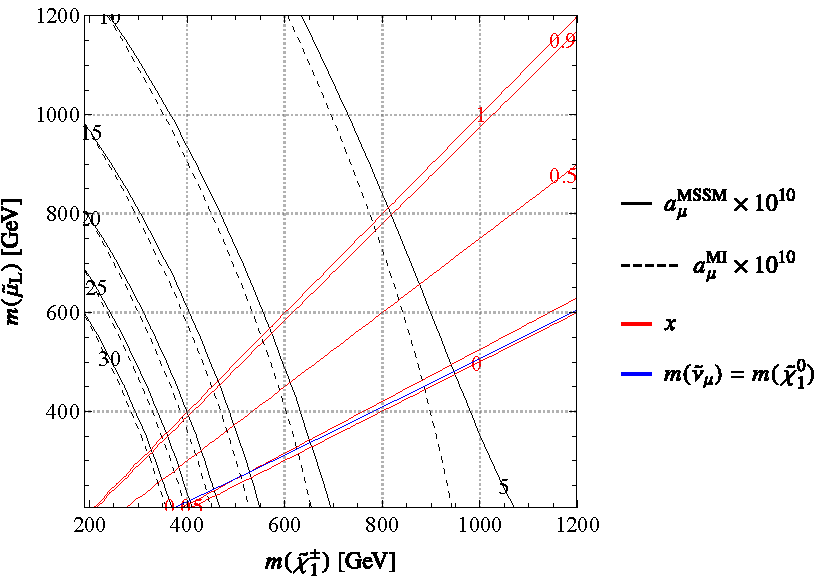
\includegraphics[scale=0.6]{../plots/plot_spectrum_tab2_physplot.pdf}
\caption{\label{fig:spectra-tab1} For $\mu=2M_2$.}
\end{subfigure}

\vspace{1em}

\begin{subfigure}[b]{\textwidth}
 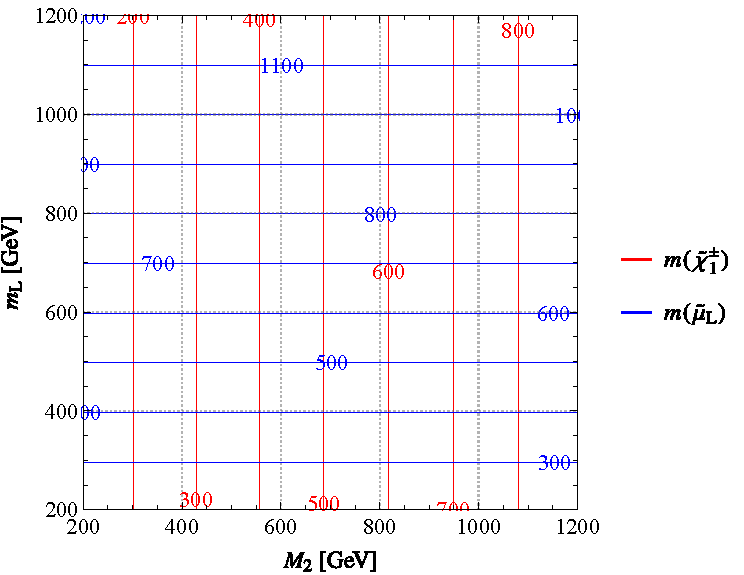
\includegraphics[scale=0.6]{../plots/plot_spectrum_tab3_massplot.pdf}
\hfill
 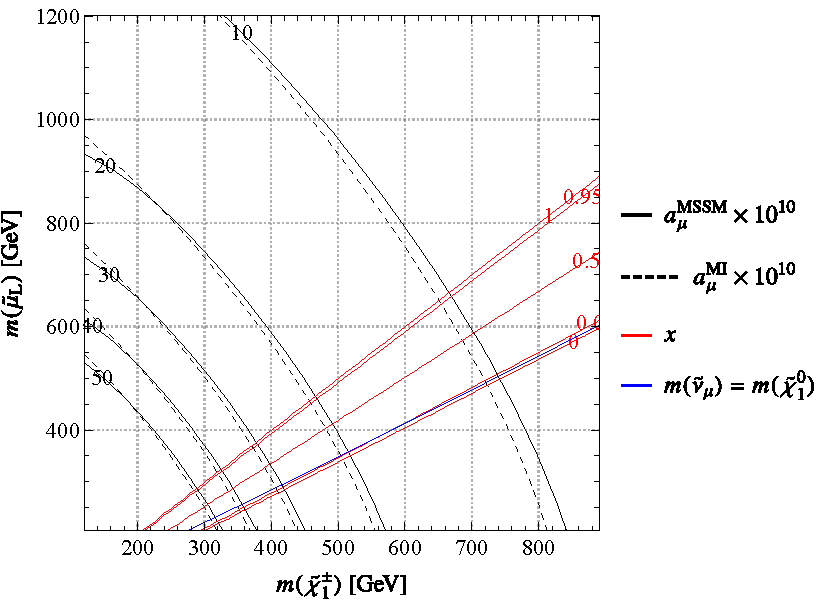
\includegraphics[scale=0.6]{../plots/plot_spectrum_tab3_physplot.pdf}
\caption{\label{fig:spectra-tab1} For $\mu=0.75M_2$.}
\end{subfigure}


\caption{\label{fig:spectra}(left) The physical mass versus soft mass parameters. (right) The muon $g-2$ values, the mass ratio $x$, and the neutralino dark matter threshold. Note that $\tilde\nu_\tau$ is slightly lighter than $\tilde\nu_\mu$ and thus it is the LSP at the region just above the blue line as well as below.}

\end{figure}





\clearpage
\appendix
\section{Formulae}
\subsection{From Endo-Hamaguchi-Iwamoto-Yanagi}
Considering the one-loop diagrams with gauge eigenstates, the SUSY contributions to the muon $g-2$ are classified into four types: BHR, BHL, BLR, and WHL, and for large $\tan\beta$ the contributions are respectively approximated as~\cite{Moroi:1995yh}
\begin{align}
  \amu[BHR]
  &= - \frac{\alpha_Y}{4\pi} \frac{m_{\mu}^2}{M_1\mu} \tan\beta\cdot
    f_N\left(\frac{M_1^2}{m_{\tilde{\mu}_R}^2}, \frac{\mu^2}{m_{\tilde{\mu}_R}^2} \right),
    \label{eq:BHR} \\
  \amu[BHL]
  &= \frac{\alpha_Y}{8\pi} \frac{m_{\mu}^2}{M_1\mu} \tan\beta\cdot
    f_N\left(\frac{M_1^2}{m_{\tilde{\mu}_L}^2}, \frac{\mu^2}{m_{\tilde{\mu}_L}^2} \right),
    \label{eq:BHL}\\
  \amu[BLR]
  &= \frac{\alpha_Y}{4\pi} \frac{m_{\mu}^2M_1\mu}{m_{\tilde{\mu}_L}^2m_{\tilde{\mu}_R}^2}
    \tan\beta\cdot
    f_N\left(\frac{m_{\tilde{\mu}_R}^2}{M_1^2}, \frac{m_{\tilde{\mu}_R}^2}{M_1^2} \right),
    \label{eq:BLR} \\
  \amu[WHL1]
  &= -\frac{\alpha_2}{8\pi} \frac{m_{\mu}^2}{M_2\mu} \tan\beta\cdot
    f_N\left(\frac{M_2^2}{m_{\tilde{\mu}_L}^2}, \frac{\mu^2}{m_{\tilde{\mu}_L}^2} \right),
    \label{eq:WHL1}\\
  \amu[WHL2]
  &= \frac{\alpha_2}{4\pi} \frac{m_{\mu}^2}{M_2\mu} \tan\beta\cdot
    f_C\left(\frac{M_2^2}{m_{\tilde{\nu}_{\mu}}^2}, \frac{\mu^2}{m_{\tilde{\nu}_{\mu}}^2} \right),
    \label{eq:WHL2}
\end{align}
where the loop functions are given by
\begin{align}
    \label{eq:loop-aprox}
    f_C(x,y)
    &=xy\left[
      \frac{5-3(x+y)+xy}{(x-1)^2(y-1)^2} - \frac{2\ln x}{(x-y)(x-1)^3}+\frac{2\ln y}{(x-y)(y-1)^3}
      \right],
    \\
    f_N(x,y)
    &= xy\left[
      \frac{-3+x+y+xy}{(x-1)^2(y-1)^2} + \frac{2x\ln x}{(x-y)(x-1)^3}-\frac{2y\ln y}{(x-y)(y-1)^3}
      \right].
\end{align}

For two-loop SUSY contributions, see Refs.~\cite{Fargnoli:2013zda,Fargnoli:2013zia,Athron:2015rva}.
\end{document}
